\section{Programmazione concorrente con OpenMP}\label{capitolo4}
OpenMP è una API multi-piattaforma per il calcolo parallelo a memoria condivisa, essa è disponibile per tutti i sistemi operativi e per i linguaggi C/C++ e Fortran. Questa API si basa su direttive del compilatore, routine di librerie e variabili d'ambiente.\\
Più in dettaglio OpenMP è un'implementazione del multi-threading, nel quale un processo \emph{master} effettua una \emph{fork} e genera un determinato numero di thread \emph{slave} sul quale suddividere il lavoro. Questi thread slave vengono eseguiti concorrentemente su differenti core o processori come mostrato in \ref{fig:openmp}.\\
\begin{figure}
\centering
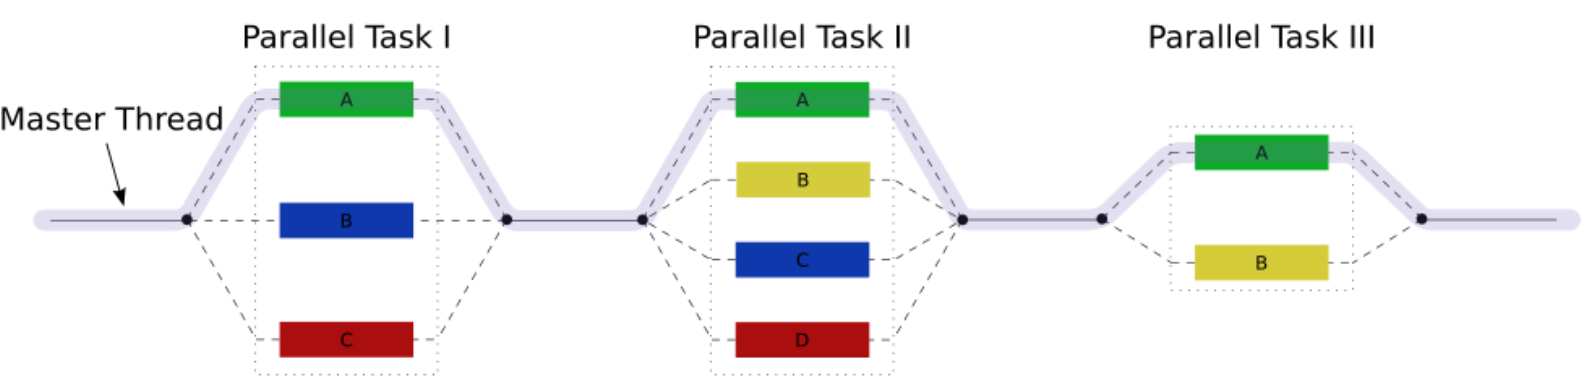
\includegraphics[width=0.7\linewidth]{img/openmp}
\caption{Suddivisione del carico tra diversi threads}
\label{fig:openmp}
\end{figure}
La maggior parte dei costrutti di OpenMP sono direttive del compilatore o \texttt{pragmas}, lo scopo principale dei questa API è quello di parallelizzare i cicli e per farlo offre un approccio incrementale al parallelismo.
Alcune peculiarità sono:
\begin{itemize}
	\item \textbf{Parallelismo innestato:} le API permettono di costruire del thread all'interno di altri thread.
	\item \textbf{Dynamic thread:} le API permettono di cambiare dinamicamente il numero di thread in esecuzione nelle differenti aree parallelizzate.
	\item \textbf{Input/Output: OpenMP} non specifica nulla riguardo agli I/O paralleli è compito del programmatore perciò assicurare la corretta esecuzione parallela.
	\item \textbf{Memory Consistency:} i threads mantengono una loro \emph{cache} e non è quindi necessario mantenere una consistenza con la memoria principale, tuttavia in caso di una variabile condivisa è responsabilità del programmatore assicurare il corretto uso della variabile.
\end{itemize}
Vediamo ora nel Listato \ref{lst:helloopen} un esempio di utilizzo delle API OpenMP
\begin{lstlisting}[language=C++,caption={Esempio di utilizzo delle OpenMP},label=lst:helloopen]
#include <omp.h>
#include <iostream>

using namespace std;
int main () {
	#pragma omp parallel num_threads(3)
	{
		cout<<"Hello World\n"
	}	
}
\end{lstlisting}
Per compilare tale codice è necessario aggiungere l'opzione \texttt{-fopenmp} al normale comando di compilazione.\\
Le direttive OpenMP valide sono identificate dal costrutto
\begin{verbatim}
		#pragma omp name [clause, ...]
\end{verbatim}
dove \emph{name} identifica la direttiva la quale può essere seguita da una o più opzioni. Una delle direttive più importanti è la direttiva \texttt{parallel} senza la quale un programma verrebbe eseguito sequenzialmente. Quando un thread raggiunge la direttiva \texttt{parallel} esso crea una team di  threads ed esso ne diventa il master. A partire dall'inizio della regione parallela il codice viene duplicato e tutti i thread eseguono lo stesso codice. Esiste un \emph{barrier} implicito alla fine della regione parallela dopo il quale solo il thread master continua l'esecuzione.
Se un thread termina all'interno di una regione parallela tutti i thread del team terminano ed l'esecuzione da quel punto è indefinita.\\
Il numero di threads da generare in una regione parallela può essere determinati da questi fattori in ordine di precedenza:
\begin{itemize}	
	\item Valutazione della clausola \texttt{if}
	\item Valore settato dalla clausola \texttt{num\_threads}
	\item L'uso della funzione di libreria \texttt{omp\_set\_num\_threads()}
	\item Il settaggio della variabile d'ambiente \texttt{OMP\_NUM\_THREADS}
	\item Implementazione e numero di CPU
\end{itemize}
La clausola \texttt{if} se valutata vera crea un team di thread altrimenti la regione viene eseguita sequenzialmente.\\
Lo standard OpenMP definisce un insieme di funzioni per determinare il numero di threads in esecuzione, bloccare l'esecuzione per scopi di sincronizzazione (semafori), definire delle routine.
Per controllare il numero di threads da creare, quelli creati e il numero di thred che stiamo eseguendo abbiamo a disposizione delle funzioni di libreria specifiche:
\begin{itemize}
	\item  \texttt{void omp\_set\_num\_threads (int num\_threads)} che imposta il numero di thread da utilizzare nelle regioni parallele, questa routine deve essere chiamata in un punto seriale del codice.
	\item \texttt{int omp\_get\_num\_threads (void)} restituisce il numero di threads che attualmente sono nel team e stanno eseguendo la regione parallela.
	\item \texttt{int omp\_get\_thread\_number (void)} restituisce il numero del thread  all'interno del team nel quale è stato chiamato, in caso in cui il chiamante sia il thread \emph{master} questa chiamata restituisce il valore $0$.
\end{itemize}
OpenMP si basa sulla un modello a memoria condivisa e molte variabile sono condivise di default, esiste tuttavia la \emph{Data Scope Attribute Clauses} che viene utilizzata per definire esplicitamente qual è lo \emph{scope} di una variabile i possibili valori che si possono assegnare sono:
\begin{itemize}
	\item private/firstprivate
	\item shared
	\item default
	\item reduction
\end{itemize}
La clausola \texttt{private} è privata in ogni thread questo significa che viene dichiarato un nuovo oggetto dello stesso tipo in ogni thread, ogni riferimento all'oggetto originale viene rimpiazzato dai riferimenti al nuovo oggetto, tuttavia si assume che tale oggetto non sia inizializzato. La clausola \texttt{firstprivate}, è simile alla clausola private ma, al contrario di questa, il valore del nuovo oggetto viene inizializzato al valore globale assunto dalla variabile prima di entrare nel blocco parallelo.
La direttiva \texttt{shared} dichiara che le variabili nella lista sono condivise tra i diversi threads del team, una variabile dichiarata \emph{shared} esiste solamente in una posizione di memoria e tutti i threads leggono e scrivono su di essa; è compito del programmatore assicurare l'integrità della variabile.\\
La clausola \texttt{default} permette al programmatore di definire lo \emph{scope} di tutte le variabili delle regioni parallele, i valori possibili sono \emph{shared} e \emph{none}, la seconda obbliga il programmatore a definire una clausola per tutte le variabili.
La direttiva \texttt{reduction} effettua una riduzione sulle variabili che compaiono nella lista, la seintassi prevede anche l'utilizzo di un operatore di riduzione. Una copia privata di ogni variabile viene creata in ogni thread ed alla fine dell'esecuzione parallela la riduzione viene applicata a tutte le copie private e il risultato viene scritto nella variabile globale.\\
La clausola \texttt{critical} specifica una regione di codice che deve essere eseguita da un thread alla volta, nel caso in cui un thread sia già all'interno di una regione critica gli altri threads devono attendere che il thread esca dalla regione, è possibile definire più di una regione critica tramite l'utilizzo di nomi per distinguere le diverse regioni.\\
Infine, la direttiva \texttt{barrier} sincronizza tutti i threads del team, quando un thread raggiunge questa direttiva attende fino a quando tutti i threads non sono arrivati alla \emph{barriera} a questo punto i threads riprendono la loro esecuzione.\\
Per un approfondimento sulle clausole e su OpenMP si rimanda a \cite{cugola:openmp} e \cite{openmp:org} mentre per un tutorial sulla programmazione si rimanda a \cite{tutorial:openmp}.